\section{Phase 5: Baseline Refinement}
\label{sec:baseline-refinement}

Following the initial baseline identification, we selected a subset of participants whose self-identified baselines aligned closely with the computed values. This selection was based on their agreement level. The selected participants included P1, P4, P6, P8, and P10. We conducted initial training using those datapoints available around baseline region. 

Subsequently, data was collected during the refinement tasks described in Paragraph~\ref{par:refineing-tasks}.Then observed about the baseline shofts. Initial and refine baseline regions are illustrated in Figure~\ref{fig:baseline-refine-all} for above participants.

\begin{figure}[h]
    \centering
    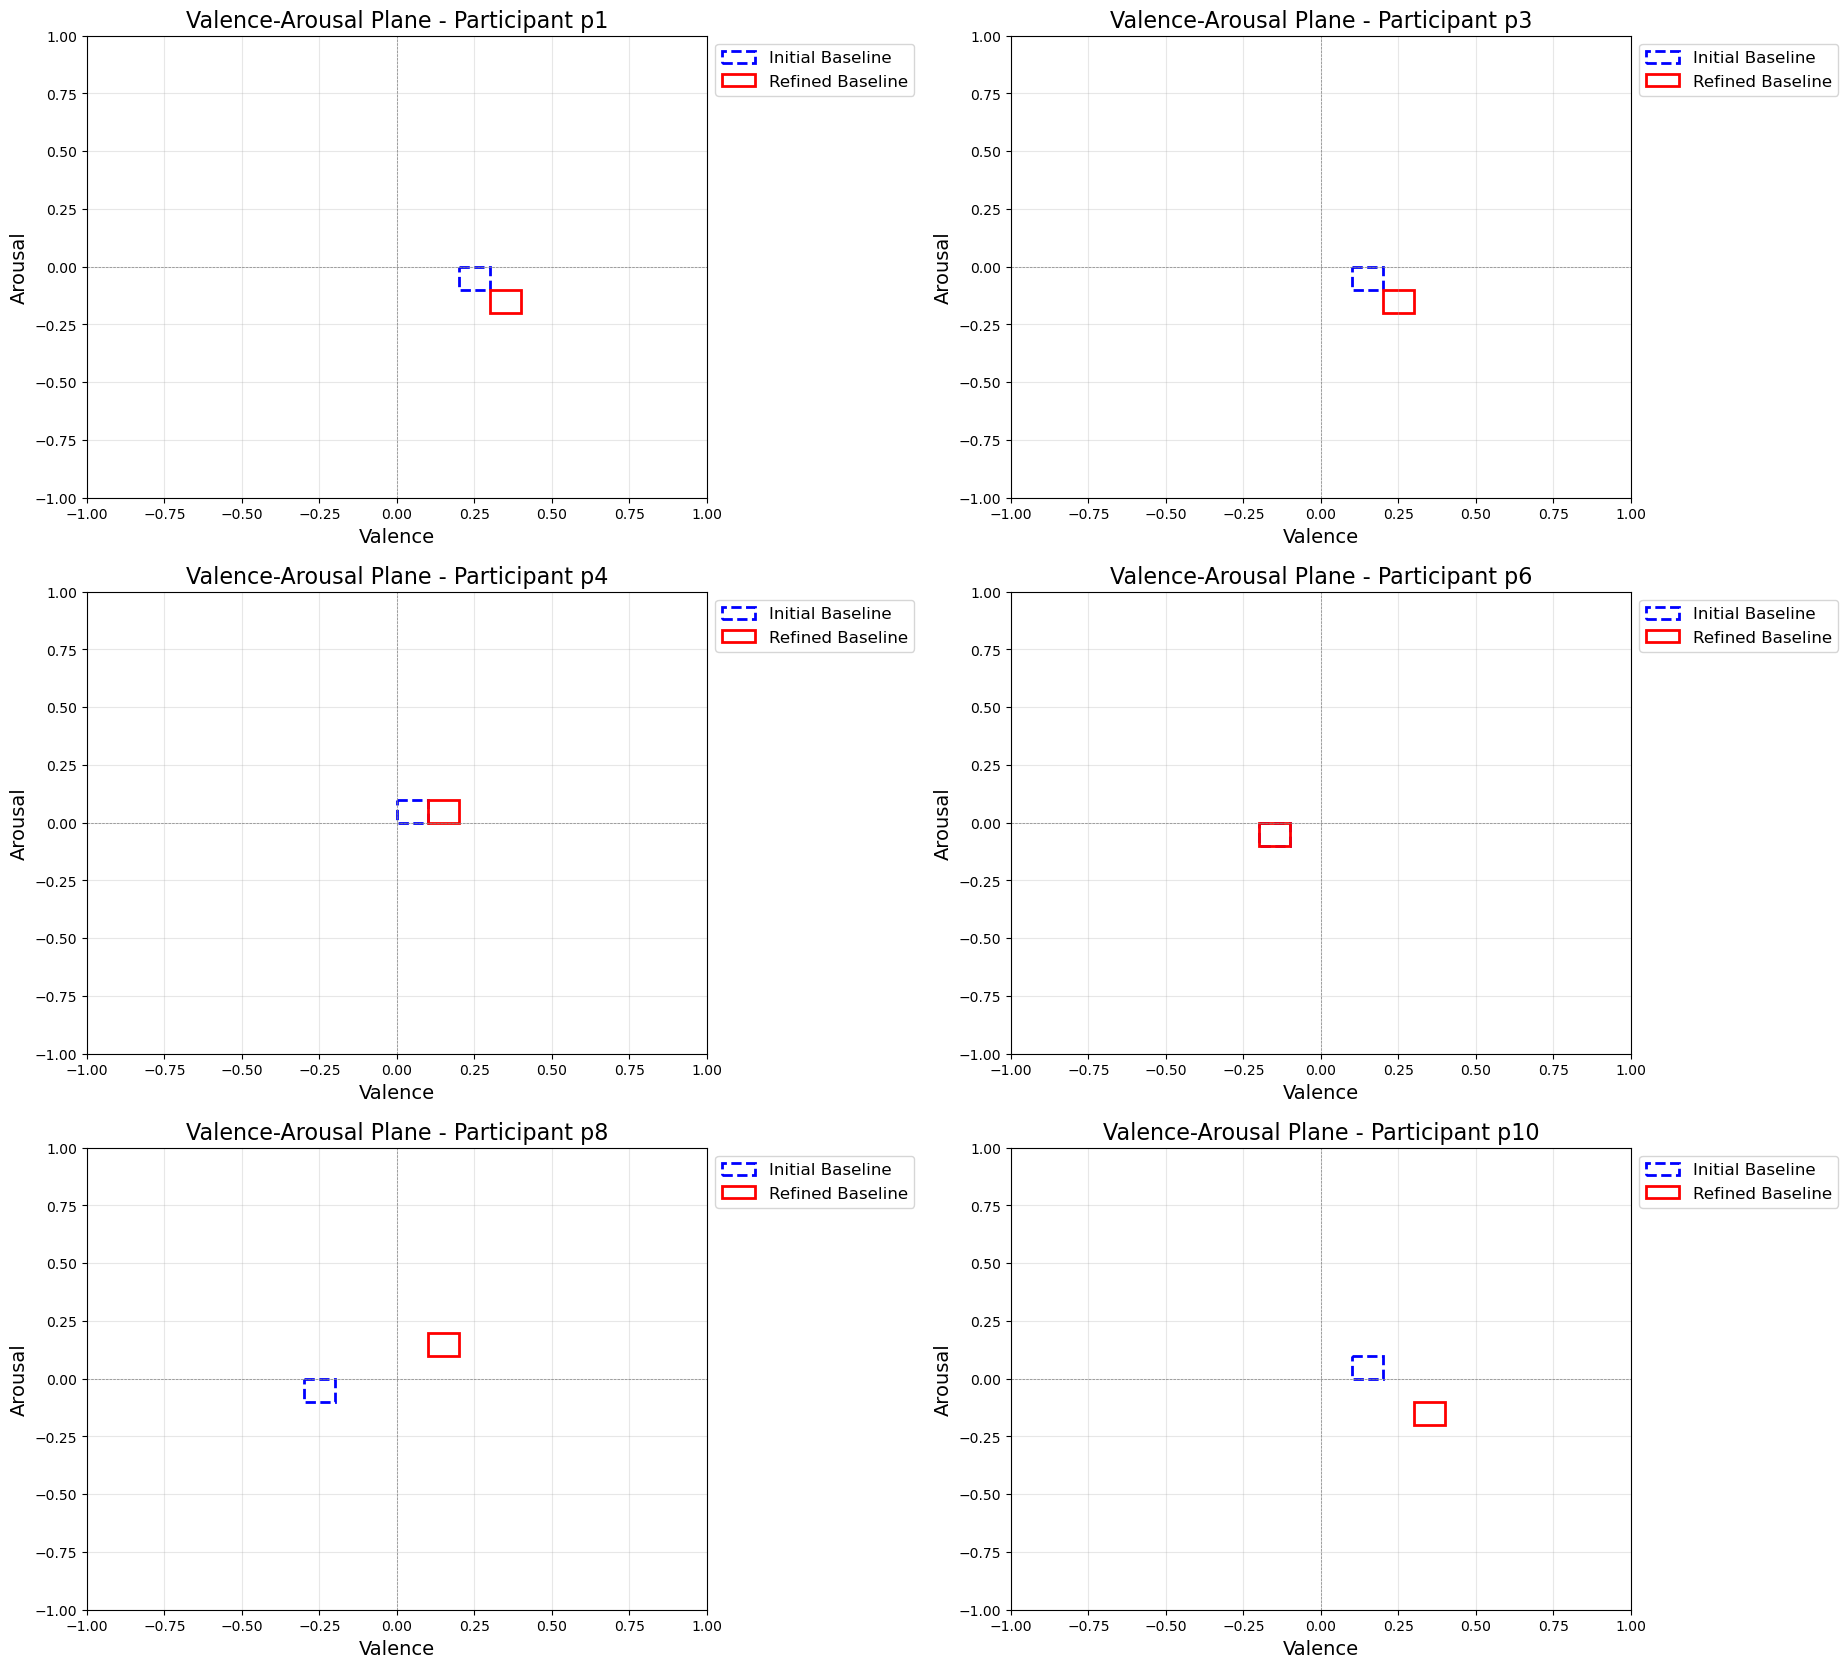
\includegraphics[width=1\textwidth]{img/chapter_04/b-refine/baseline-refine-all.png}
    \caption{Initial and refined baseline regions for selected participants.}
    \label{fig:baseline-refine-all}
\end{figure}


The results of this section are detailed in Appendix \ref{sec:appendix-refine-questionnaire}, where participant feedback on the refined baselines was collected. As shown in the table, the agreement scores and refined baseline coordinates were evaluated using a Likert scale. Out of the six participants, four (P1, P3, P4, and P6) rated the refined baselines with a score of 4 or higher, indicating agreement with the computed values. This reflects a 66.67\% agreement rate, suggesting that the refined baseline identification method was successful for the majority of users.

\begin{table}[H]
\centering
\caption{Participant Agreement on Refined Baselines}
\begin{tabular}{|c|p{5cm}|c|}
\hline
\textbf{PID} & \textbf{Refined Baseline (V, A)} & \textbf{Likert Score} \\
\hline
P1 & [(0.3, -0.1), (0.4, -0.2)] & 4 \\
P3 & [(0.2, -0.1), (0.3, -0.2)] & 5 \\
P4 & [(0.1, 0.1), (0.2, 0.0)] & 5 \\
P6 & [(-0.2, 0.0), (-0.1, -0.1)] & 4 \\
P8 & [(0.1, 0.2), (0.2, 0.1)] & 2 \\
P10 & [(0.3, -0.1), (0.4, -0.2)] & 3 \\
\hline
\end{tabular}
\end{table}